\chapter{Manipulation of HBase}
%Intro\footnotemark\\
\par After finalize the Configuring of Hbase, we will manipulate a database with the interactive shell, so we let's hbase shell and start manipulating.
\\
\begin{spacing}{1.2}
%note en bas de page
\section{Creation of a BD }
\par Create the table and associated column families and Checking that the table is created correctly.
\\
\begin{figure}[!htb] 
\begin{center} 
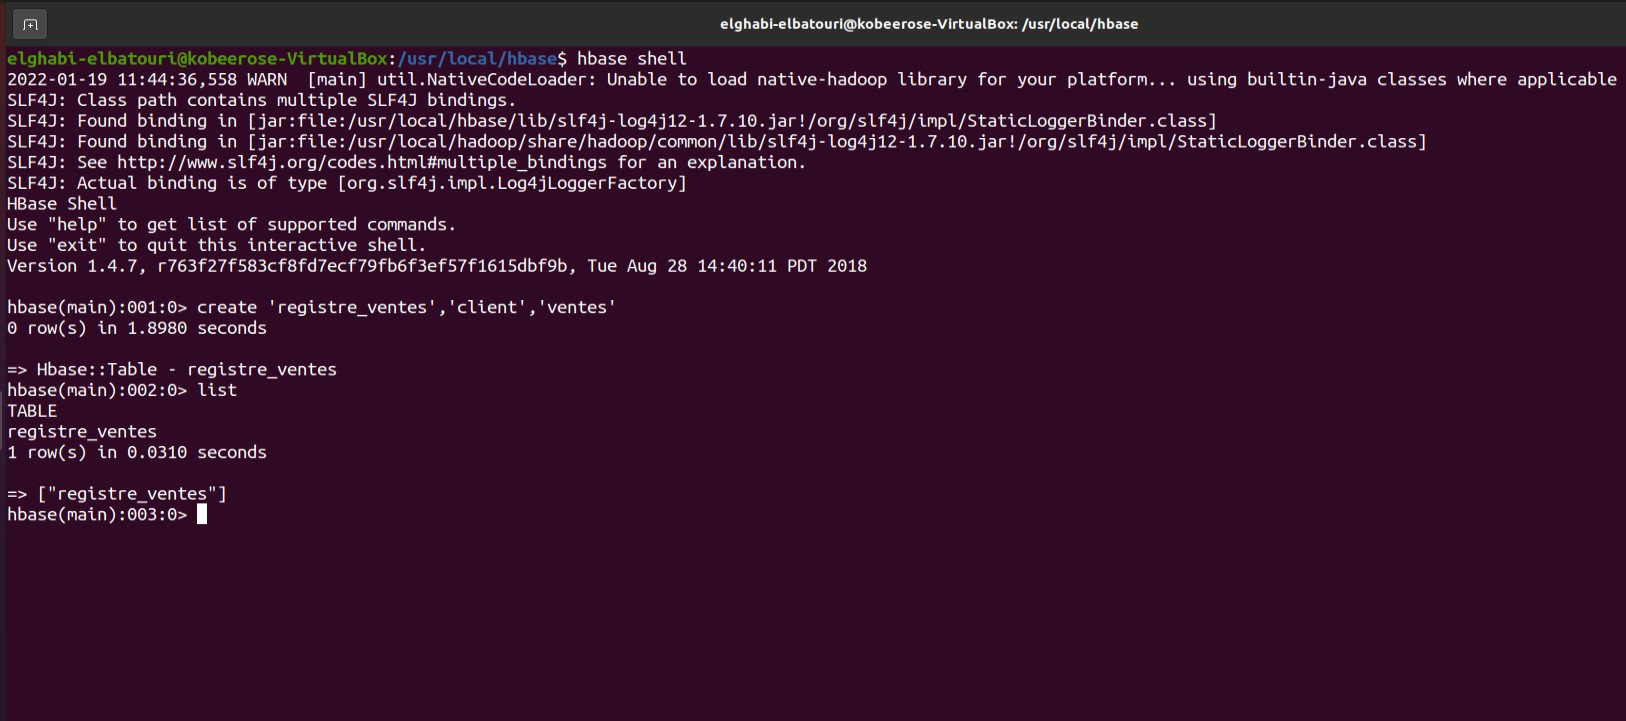
\includegraphics[width=1\linewidth]{Pictures/HBase/Manipulation of HBase/Creation of a BD/Creating a table and Verifying .jpg} 
\end{center} 
\caption{Creating a table and Verifying } 
\end{figure}  \FloatBarrier
\\
\newpage

\par Inserting the different rows of the “registre\_sales” table.
\\
\begin{figure}[!htb] 
\begin{center} 
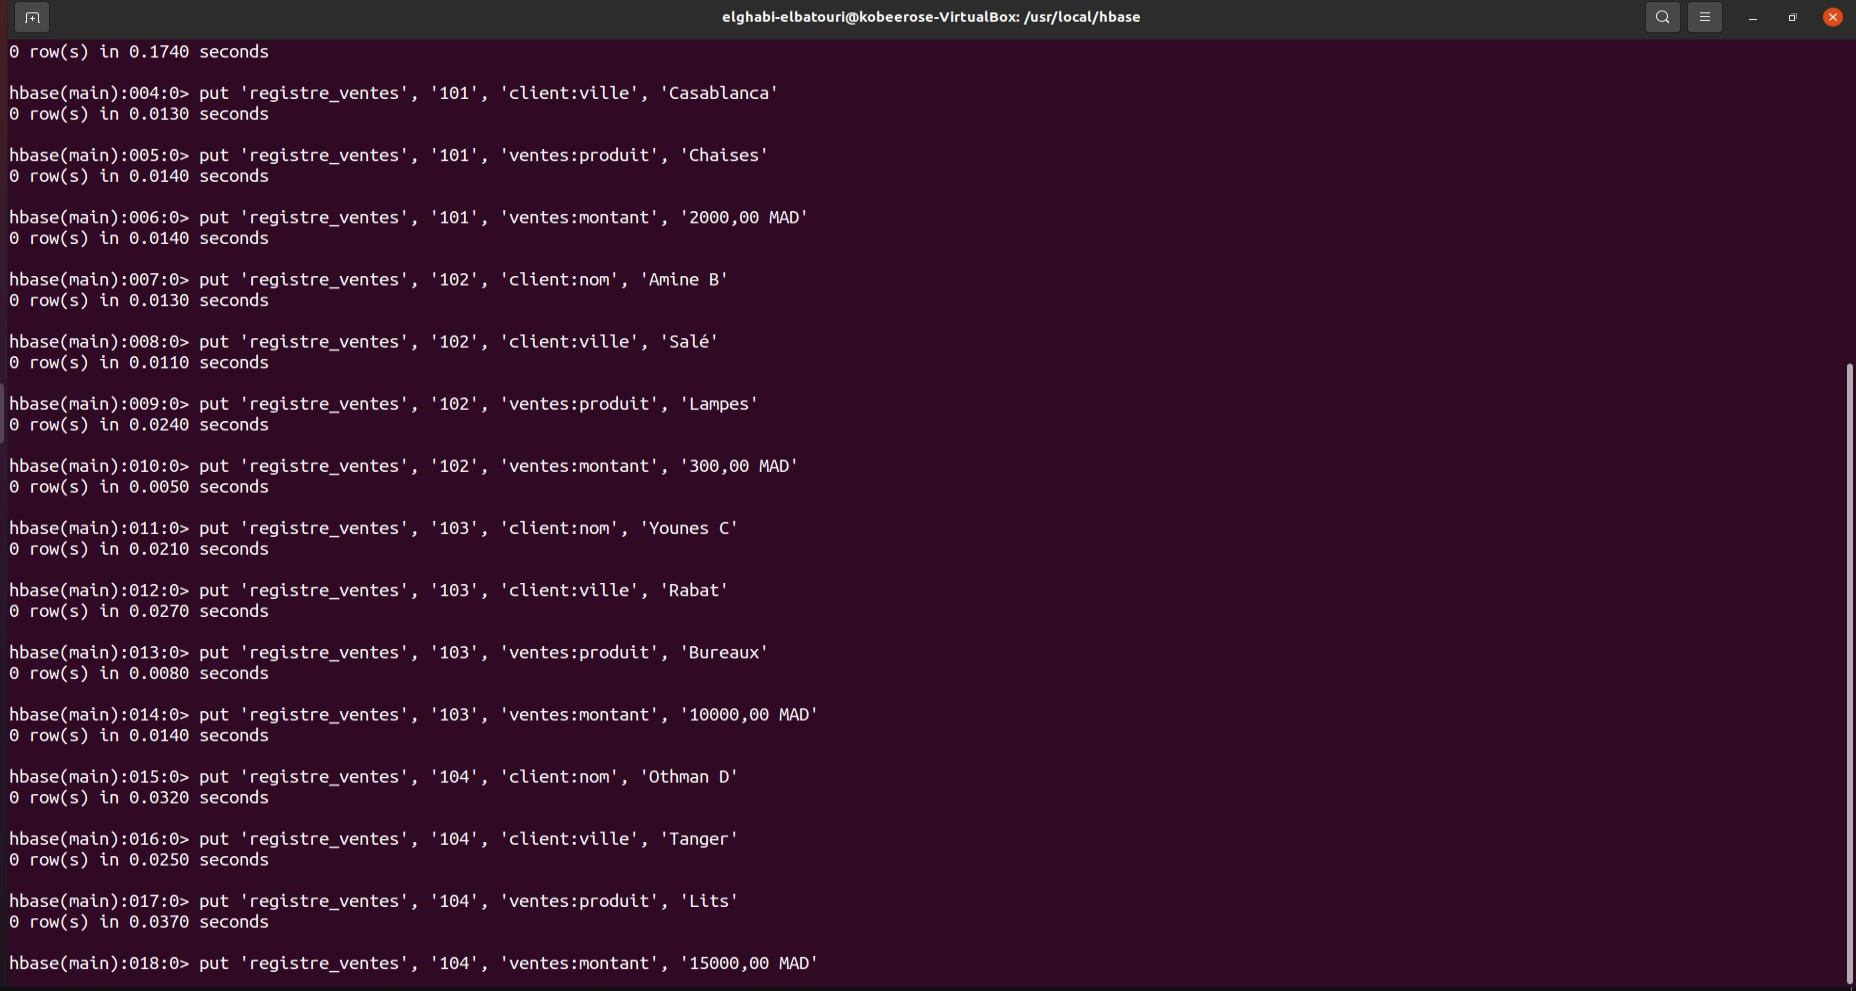
\includegraphics[width=1\linewidth]{Pictures/HBase/Manipulation of HBase/Creation of a BD/Inserting Values to the table} 
\end{center} 
\caption{Inserting Values to the table} 
\end{figure}  \FloatBarrier
\\

\par Visualize the result of the insertion in the table.
\\
\begin{figure}[!htb] 
\begin{center} 
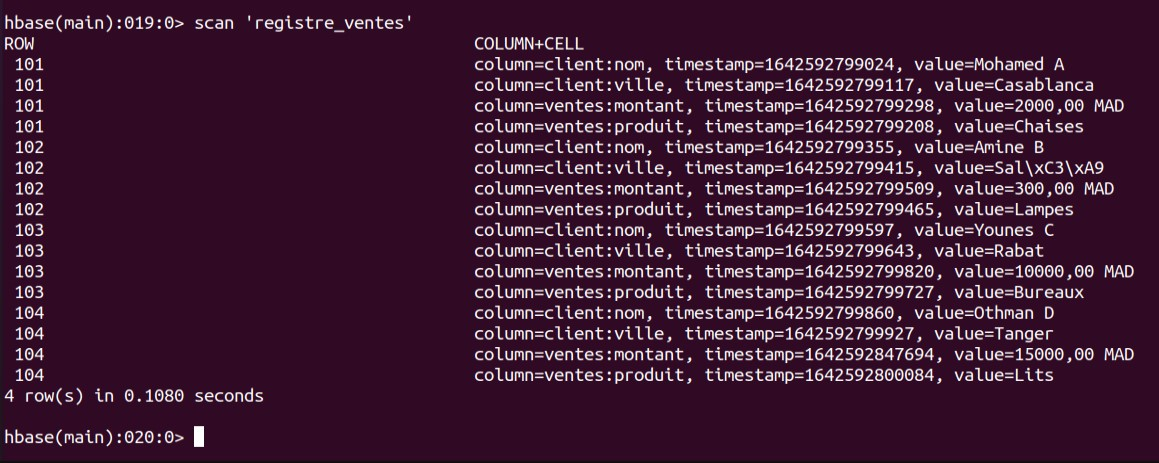
\includegraphics[width=1\linewidth]{Pictures/HBase/Manipulation of HBase/Creation of a BD/Checking the table} 
\end{center} 
\caption{Checking the table} 
\end{figure}  \FloatBarrier
\\
\newpage
\par Display the values of the "product" column of row 102.
\\
\begin{figure}[!htb] 
\begin{center} 
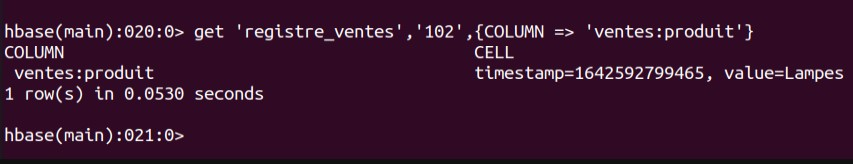
\includegraphics[width=1\linewidth]{Pictures/HBase/Manipulation of HBase/Creation of a BD/Display values of row 102} 
\end{center} 
\caption{Display values of row 102} 
\end{figure}  \FloatBarrier
\\

\par To delete a table, we can use the commands disable then drop.
\\
\begin{figure}[!htb] 
\begin{center} 
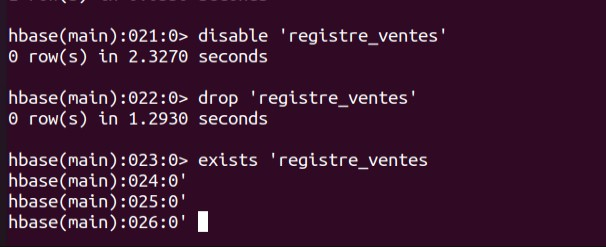
\includegraphics[width=1\linewidth]{Pictures/HBase/Manipulation of HBase/Creation of a BD/Droping a table} 
\end{center} 
\caption{Droping a table} 
\end{figure}  \FloatBarrier
\\

\end{spacing}